% ==============================================================================
% SECCIÓN 8: DISEÑO DE INTERFACES DE USUARIO (DESKTOP Y RESPONSIVE 360PX)
% ==============================================================================

\section{Diseño de Interfaces de Usuario (UI/UX)}

El diseño visual del sistema web SYSELL ha sido concebido bajo un enfoque \textbf{Responsive y Mobile-First}, asegurando que todas las vistas operativas (Punto de Venta, Inventario, Reportes y Usuarios) mantengan una ergonomía y usabilidad óptimas tanto en terminales de escritorio (1920$\times$1080px) como en dispositivos móviles compactos de mostrador (\textbf{Vista Responsive 360px}).

\subsection{Módulo de Autenticación e Inicio de Sesión}

\begin{figure}[H]
\centering
\begin{subfigure}[b]{0.62\textwidth}
    \centering
    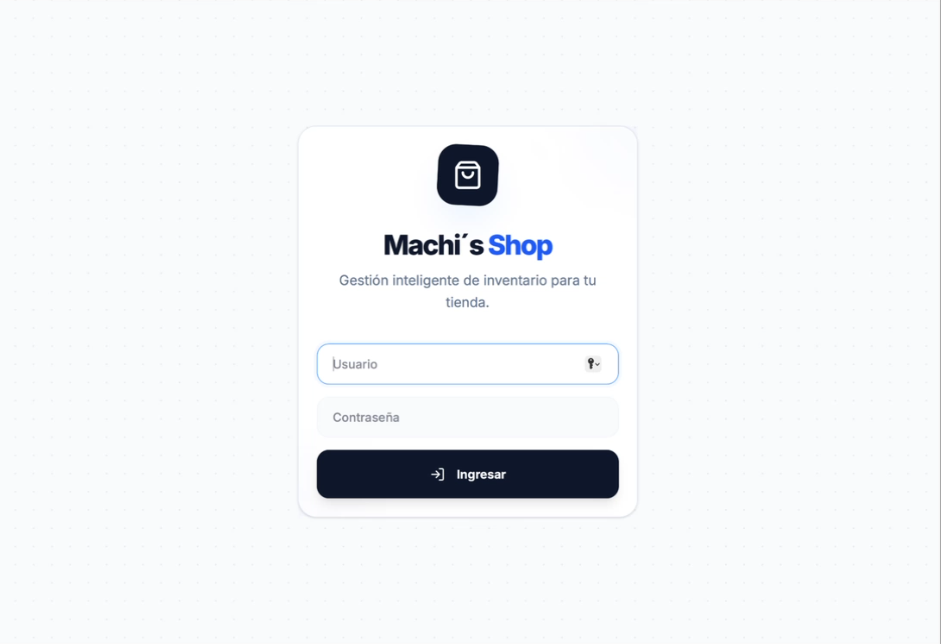
\includegraphics[width=\textwidth]{figures/mockup_login_desktop.png}
    \caption{Vista Escritorio (Desktop --- 1920px).}
    \label{fig:login_desktop}
\end{subfigure}
\hfill
\begin{subfigure}[b]{0.32\textwidth}
    \centering
    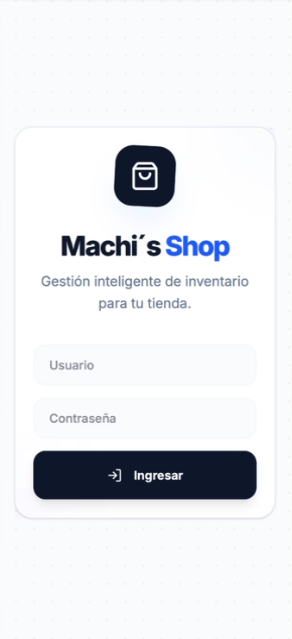
\includegraphics[width=\textwidth]{figures/mockup_login_mobile.png}
    \caption{Vista Responsive (360px).}
    \label{fig:login_mobile}
\end{subfigure}
\caption{Interfaz de Inicio de Sesión y Autenticación del Sistema SYSELL.}
\label{fig:mockup_login}
\end{figure}

\subsection{Módulo de Gestión y Registro de Usuarios}

\begin{figure}[H]
\centering
\begin{subfigure}[b]{0.62\textwidth}
    \centering
    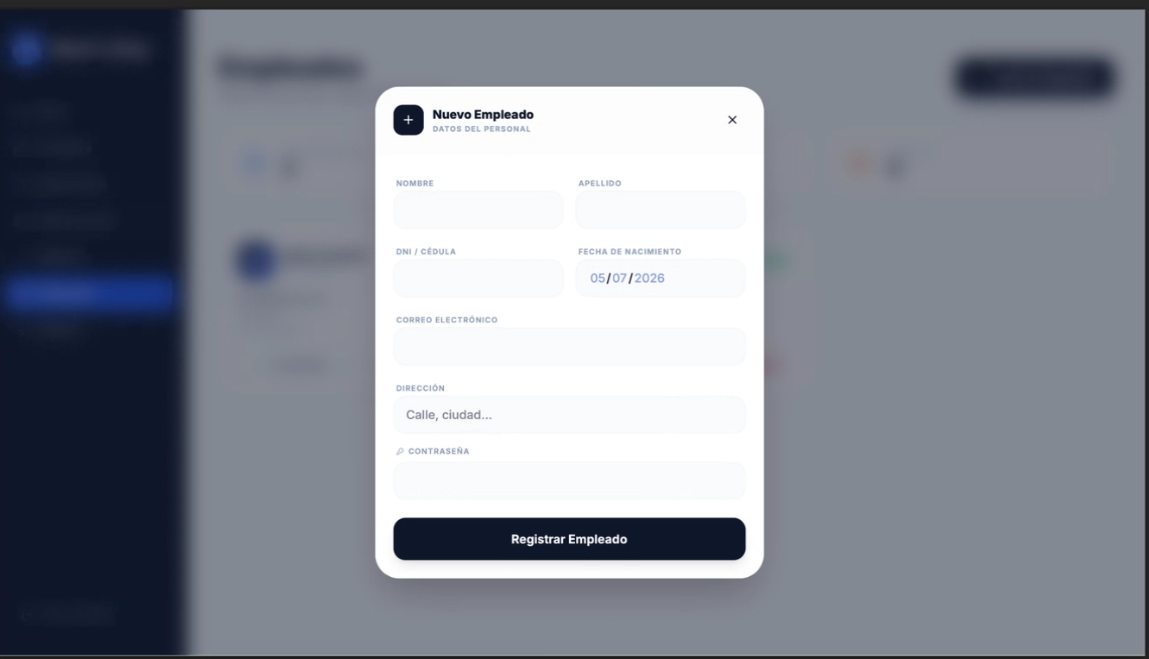
\includegraphics[width=\textwidth]{figures/mockup_usuarios_desktop.png}
    \caption{Vista Escritorio (Desktop --- 1920px).}
    \label{fig:usuarios_desktop}
\end{subfigure}
\hfill
\begin{subfigure}[b]{0.32\textwidth}
    \centering
    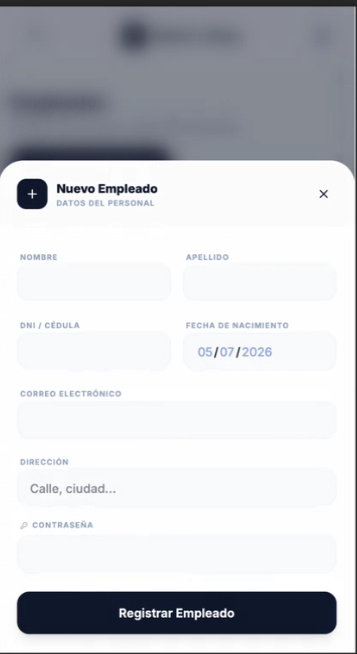
\includegraphics[width=\textwidth]{figures/mockup_usuarios_mobile.png}
    \caption{Vista Responsive (360px).}
    \label{fig:usuarios_mobile}
\end{subfigure}
\caption{Interfaz de Administración de Empleados y Control de Roles.}
\label{fig:mockup_usuarios}
\end{figure}

\subsection{Módulo de Punto de Venta (POS) y Registro de Ventas}

\begin{figure}[H]
\centering
\begin{subfigure}[b]{0.58\textwidth}
    \centering
    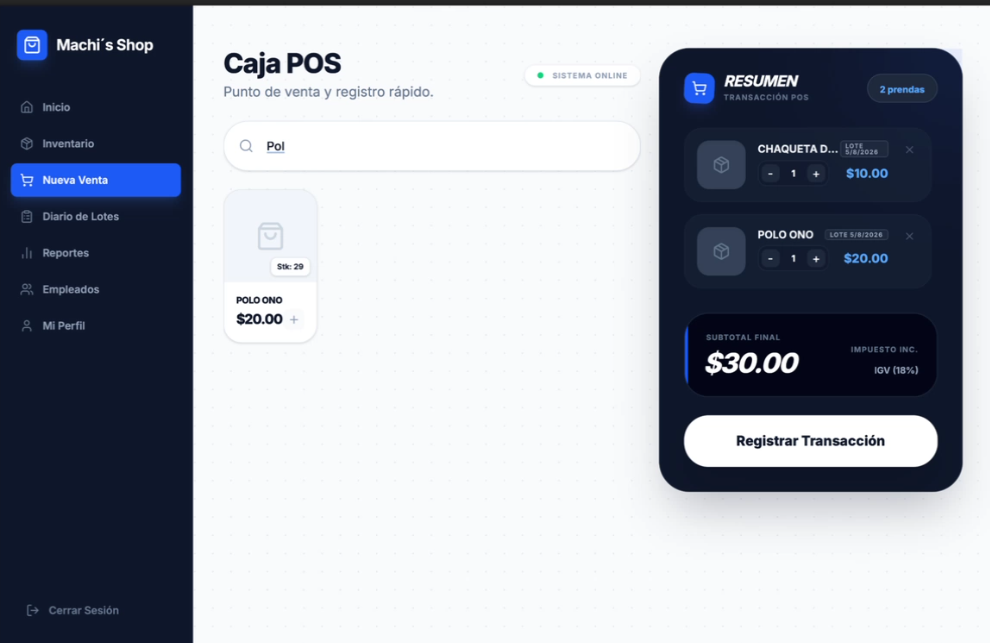
\includegraphics[width=\textwidth]{figures/mockup_ventas_desktop.png}
    \caption{Vista Escritorio (Desktop --- Punto de Venta Mostrador).}
    \label{fig:ventas_desktop}
\end{subfigure}
\hfill
\begin{subfigure}[b]{0.19\textwidth}
    \centering
    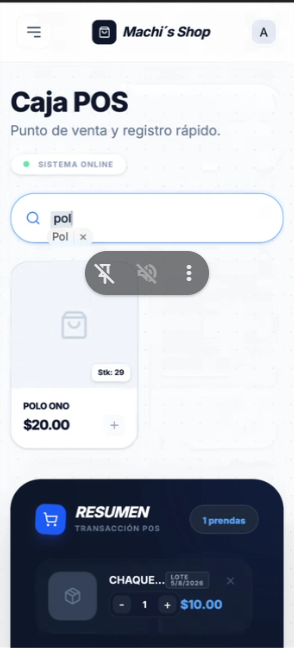
\includegraphics[width=\textwidth]{figures/mockup_ventas_mobile_1.png}
    \caption{Vista Responsive (360px) --- Catálogo.}
    \label{fig:ventas_mobile_1}
\end{subfigure}
\hfill
\begin{subfigure}[b]{0.19\textwidth}
    \centering
    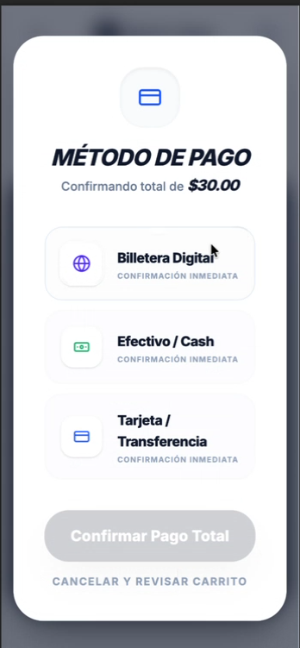
\includegraphics[width=\textwidth]{figures/mockup_ventas_mobile_2.png}
    \caption{Vista Responsive (360px) --- Carrito.}
    \label{fig:ventas_mobile_2}
\end{subfigure}
\caption{Interfaz del Módulo de Ventas y Carrito de Compras en Mostrador.}
\label{fig:mockup_ventas}
\end{figure}

\subsection{Módulo de Inventario, Catálogo y Control de Stock}

\begin{figure}[H]
\centering
\begin{subfigure}[b]{0.62\textwidth}
    \centering
    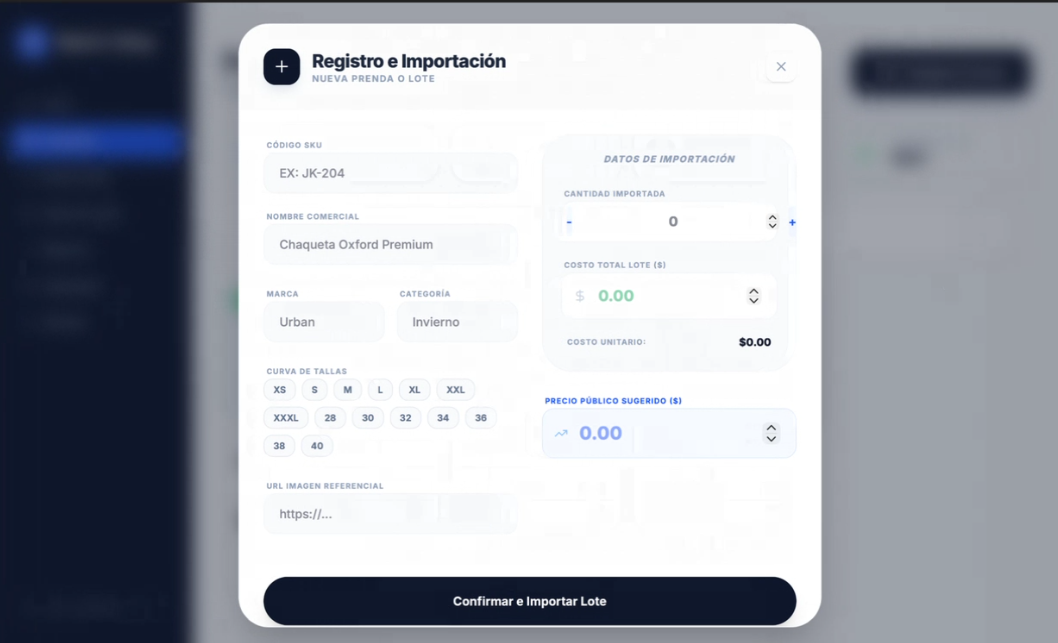
\includegraphics[width=\textwidth]{figures/mockup_inventario_desktop.png}
    \caption{Vista Escritorio (Desktop --- Tabla de Productos y Variantes).}
    \label{fig:inventario_desktop}
\end{subfigure}
\hfill
\begin{subfigure}[b]{0.32\textwidth}
    \centering
    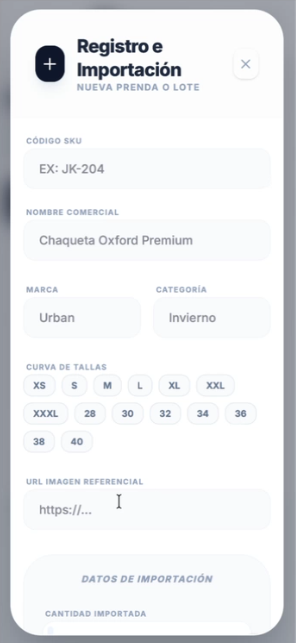
\includegraphics[width=\textwidth]{figures/mockup_inventario_mobile.png}
    \caption{Vista Responsive (360px).}
    \label{fig:inventario_mobile}
\end{subfigure}
\caption{Interfaz de Gestión de Inventario, Precios y Stock Mínimo.}
\label{fig:mockup_inventario}
\end{figure}

\subsection{Módulo de Reportes, Analítica y Balances Financieros}

\begin{figure}[H]
\centering
\begin{subfigure}[b]{0.62\textwidth}
    \centering
    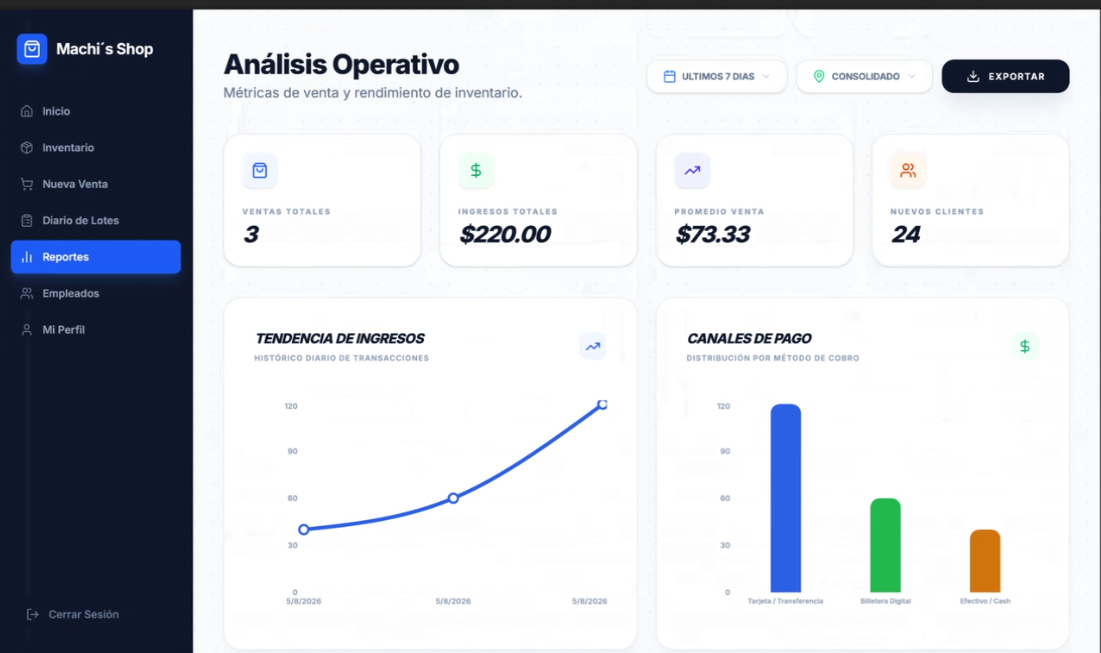
\includegraphics[width=\textwidth]{figures/mockup_reportes_desktop.png}
    \caption{Vista Escritorio (Desktop --- Gráficos y Tablas Consolidadas).}
    \label{fig:reportes_desktop}
\end{subfigure}
\hfill
\begin{subfigure}[b]{0.32\textwidth}
    \centering
    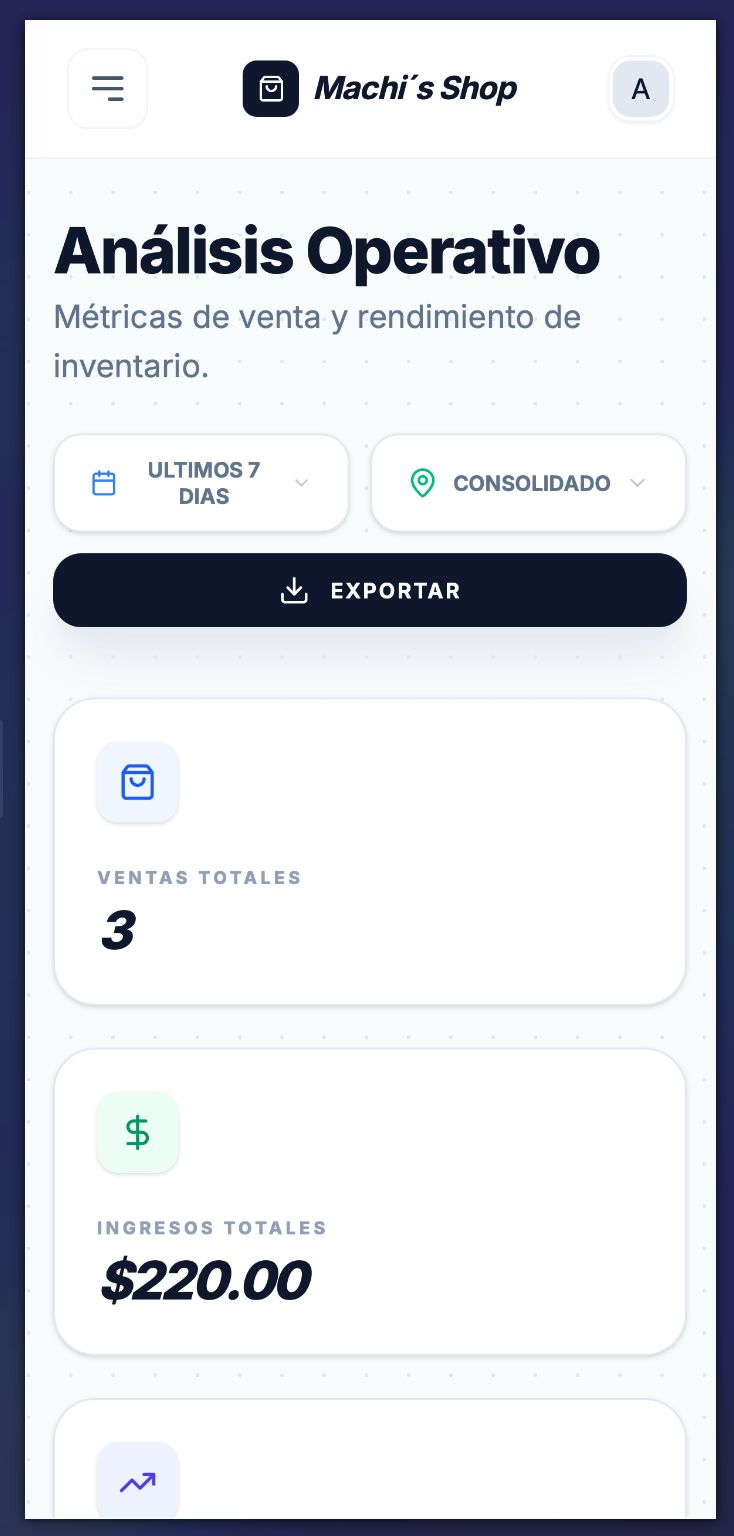
\includegraphics[width=\textwidth]{figures/mockup_reportes_mobile.png}
    \caption{Vista Responsive (360px).}
    \label{fig:reportes_mobile}
\end{subfigure}
\caption{Interfaz de Reportes Analíticos, Filtrado Temporal y Exportación.}
\label{fig:mockup_reportes}
\end{figure}

\subsection{Diagrama de Navegabilidad y Flujo de Pantallas}

\begin{figure}[H]
\centering
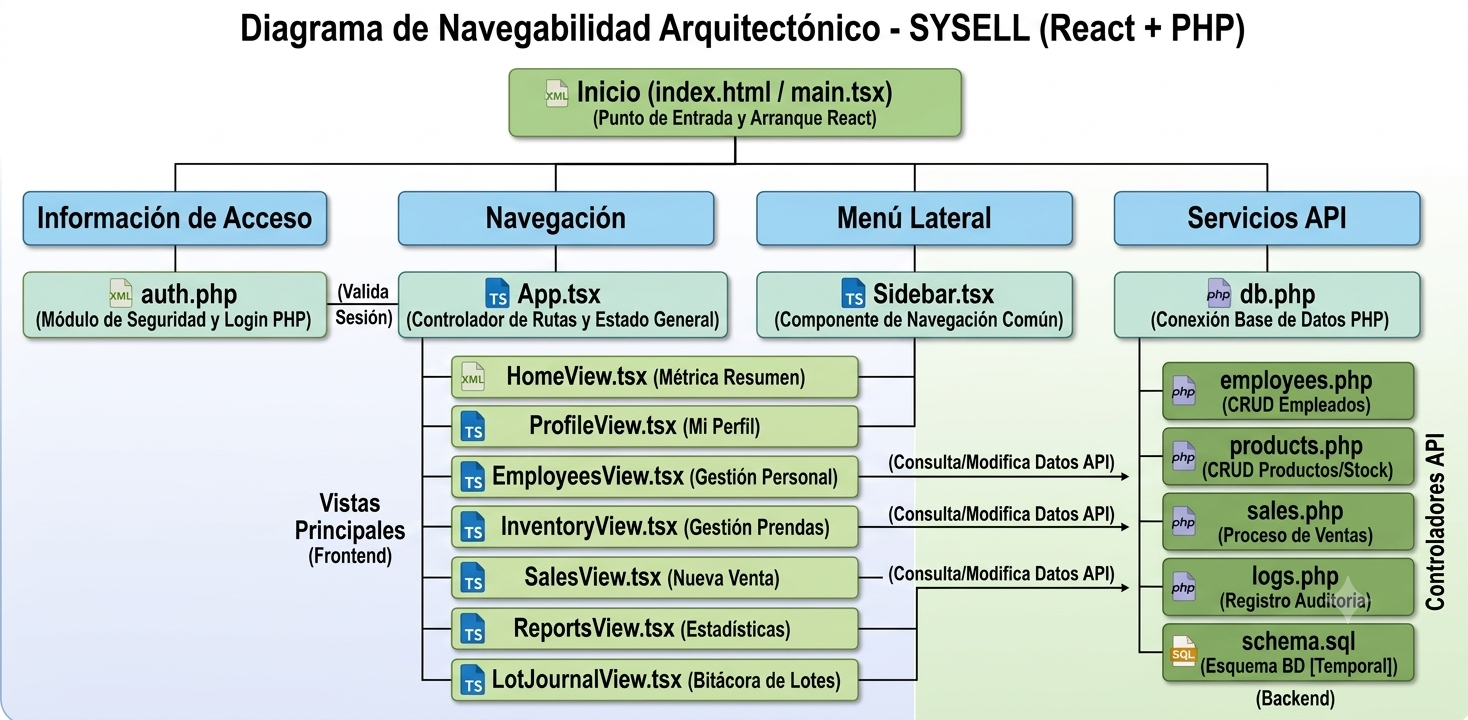
\includegraphics[width=0.85\linewidth]{figures/diagrama_navegabilidad.png}
\caption{Diagrama de Navegabilidad y Flujo de Vistas del Sistema SYSELL.}
\label{fig:diagrama_navegabilidad}
\end{figure}
